\documentclass{beamer}
\usetheme{metropolis}
\usepackage{graphicx}
\usepackage{subfig}
\usepackage{tcolorbox}
\title{Algebra-Based Physics-2: Electricity, Magnetism, and Modern Physics (PHYS135B): Unit 0}
\author{Jordan Hanson}
\institute{Whittier College Department of Physics and Astronomy}

\begin{document}
\maketitle

\begin{frame}{Course Introduction}
\begin{enumerate}
\item Professor Jordan Hanson
\item Contact: jhanson2@whittier.edu, SLC 212
\item Syllabus: Moodle
\item Office hours: Book appointment online
\item PHYS135A is pre-requisite
\item Text: College Physics (openstax.org), see link on syllabus.
\item Homework: OpenStax Tutor, \$10.00
\end{enumerate}
\end{frame}

\section{Summary}

\begin{frame}{Unit 0 Summary}
\textit{Physics} - $\phi\upsilon\sigma\iota\kappa\acute{\eta}$ - "phusik\'e": \textit{knowledge of nature} \\
from $\phi\acute{\upsilon}\sigma\iota\varsigma$ - "ph\'usis": \textit{nature} \\
\textbf{Reading: Chapters 18 and 19 (for Unit 1)}
\begin{enumerate}
\item Estimation/Approximation
\item Review of concepts from Newtonian mechanics
\begin{itemize}
\item Kinematics and \alert{Newton's Laws}
\item Work-energy theorem, energy conservation
\item Momentum, conservation of momentum
\end{itemize}
\item Charge
\begin{enumerate}
\item Types of charge, charge conservation
\item Couloumb force
\item Electric fields
\end{enumerate}
\end{enumerate}
\end{frame}

\begin{frame}{Bonus Essay}
\small
\textbf{\alert{Bonus Essay assignment}}: Students may submit an essay on the history of scientific developments covered in the course, due at the end of the semester. The essay must be 10 pages, address scientific arguments and results, and must include references. The grade of this paper will replace the lowest midterm grade, if it would raise the final grade.  Example topics:
\begin{itemize}
\item Measurement of cosmic ray flux by Victor Hess
\item Discovery of the charge to mass ratio of the electron by J.J. Thompson
\item First description of the \textit{photoelectric effect} by Albert Einstein
\end{itemize}
(Before beginning the essay, please discuss it with me in office hours).
\end{frame}

\section{Estimation/Approximation}

\begin{frame}{Estimation/Approximation}
In science and engineering, \alert{estimation} is to obtain a quantity in the absence of precision, informed by rational constraints.
\begin{enumerate}
\item Define relevant \alert{unit scales}: (mg, g, or kg), (m/s or km/hr)
\item Obtain \alert{complex quantities} from simple ones
\begin{itemize}
\item Obtain \textit{areas} and \textit{volumes} from \textit{lengths}
\item Obtain \textit{rates} from \textit{numerators} and \textit{denominators}
\end{itemize}
\item \textbf{Scaling problems: how does a complex quantity depend on other quantities?}
\item Constrain the unknown with \alert{upper} and \alert{lower} limits
\end{enumerate}
(Professor: work an example of each on the board).
\end{frame}

\begin{frame}{WAT.}
\centering

\includegraphics[width=0.7\textwidth]{figures/watduck.jpeg}
\end{frame}

\begin{frame}{WAT.}
\centering
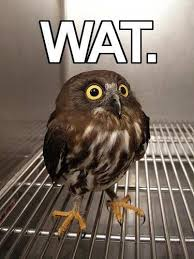
\includegraphics[width=0.4\textwidth]{figures/watowl.jpeg}
\end{frame}

\begin{frame}{Estimation/Approximation}
\textbf{Unit scale}: The distance between the Earth and the sun is 1 AU.  What is the distance between the Sun and Venus?
\begin{itemize}
\item A: 10 million km
\item B: 100 million km
\item C: 0.2 AU
\item D: 0.7 AU
\end{itemize}
\end{frame}

\begin{frame}{Estimation/Approximation}
\textbf{Unit scale}: The distance around a track is 400 m.  Which of the following is the time it takes a fast runner to proceed all the way around the track?
\begin{itemize}
\item A: 4 seconds
\item B: 0.1 minutes
\item C: 1.0 minute
\item D: 20 minutes
\end{itemize}
\end{frame}

\begin{frame}{Estimation/Approximation}
\textbf{Volumes from other quantities}: How many grains of rice are there in a bag?  Assume the bag is 10 cm x 10 cm x 5 cm.  Assume a grain of rice is 0.4 cm x 0.3 cm x 0.3 cm.
\vspace{0.55cm}
\begin{itemize}
\item A: 1500
\item B: 15,000
\item C: 150,000
\item D: Many.
\end{itemize}
\end{frame}

\begin{frame}{Estimation/Approximation}
\textbf{Rates from other quantities}: A student travels from uptown Whittier to SLC in roughly 10 minutes.  What is her average speed?
\begin{itemize}
\item A: 0.1 m/s
\item B: 0.33 m/s
\item C: 1.33 m/s
\item D: 10 m/s
\end{itemize}
\end{frame}

\begin{frame}{Estimation/Approximation}
\textbf{Scaling problem}: If the \textit{temperature} of a gas remains constant, the \textit{pressure} is inversely proportional to the volume of the gas.  If the volume of a cylinder is \textit{decreased} by a factor of three, by what factor does the pressure change, if the temperature remains the same?
\begin{itemize}
\item A: 3
\item B: 1/3
\item C: 1
\item D: 9
\end{itemize}
\end{frame}

\begin{frame}{Estimation/Approximation}
\textbf{Scaling problem}: The gravitational pull between two massive objects is inversely proportional to the \textit{distance squared} between them.  By what factor does the force of gravity between two objects change if the distance between them is \textit{decreased} by a factor of 2.0?
\begin{itemize}
\item A: 2.0
\item B: 0.5
\item C: 4.0
\item D: 0.25
\end{itemize}
\end{frame}

\begin{frame}{Estimation/Approximation}
\textbf{Constrain the unknown with lower and upper limits}: How many books are there in Wardman Library? \\ \vspace{0.5cm}
\textbf{This is a group board problem.  Complete this estimation with your group.} \\ \vspace{0.5cm}
(Professor: white board space...)
\end{frame}

\begin{frame}{Coordinates and Vectors}
\small
\begin{columns}[T]
\begin{column}{0.5\textwidth}
$\vec{p} = 4\hat{i}+2\hat{j}$.  $\vec{q} = -4\hat{i}+2\hat{j}$.  \\
Compute $\vec{p} + \vec{q}$.
\vspace{0.2cm}
\begin{itemize}
\item A: $4\hat{i}+4\hat{j}$
\item B: $0\hat{i}+4\hat{j}$
\item C: $4\hat{i}+0\hat{j}$
\item D: 0
\end{itemize}
\end{column}
\begin{column}{0.5\textwidth}
$\vec{p} = -1\hat{i}+6\hat{j}$.  $\vec{q} = 3\hat{i}+0.5\hat{j}$.  \\
Compute $\vec{p} \cdot \vec{q}$.
\vspace{0.2cm}
\begin{itemize}
\item A: -1
\item B: 1
\item C: 0
\item D: 3
\end{itemize}
\end{column}
\end{columns}
\end{frame}

\section{Kinematics and Newton's Laws}

\begin{frame}{Kinematics and Newton's Laws}
\small
\textit{Kinematics} - A \alert{description} of the motion of particles and systems \\
\textit{Dynamics} - An \alert{explanation} of the motion of particles and systems \\
\vspace{0.25cm}
What causes an object to move?  \textbf{Forces}.  Forces exist as a result of the \alert{\textbf{interactions}} of objects or systems.\\
\vspace{0.25cm}
\rule{10cm}{0.4pt} \\
\vspace{0.25cm}
\textit{Evolution} - A \alert{description} of the change of biological species \\
\textit{Natural Selection} - An \alert{explanation} of change in biological species \\
\vspace{0.25cm}
What causes species to evolve?  \textbf{Natural selection}.  Natural selection exists because of \alert{election pressures}, \alert{numerous offspring}, and \alert{variation} among offspring.
\end{frame}

\begin{frame}{Kinematics and Newton's Laws}
\textbf{Newton's First Law}: A man slides a palette crate across a concrete floor of his shop.  He exerts a force of 60.0 N, and the box has a constant velocity of 0.5 m/s.  What force cancels his pushing force, and what is the value in Newtons?
\begin{itemize}
\item A: wind, 60.0 N
\item B: friction: 60.0 N
\item C: friction: -60.0 N
\item D: weight: -60.0 N
\end{itemize}
\end{frame}

\begin{frame}{Kinematics and Newton's Laws}
\textbf{Newton's Second Law}: The crate has a mass of 50 kg, and encounters an area where there is no longer friction.  If the pushing force is still 60 N, what is the acceleration?
\begin{itemize}
\item A: 1.0 m/s$^2$
\item B: 0.8 m/s
\item C: 1.2 m/s
\item D: 1.2 m/$^2$
\end{itemize}
\end{frame}

\begin{frame}{Kinematics and Newton's Laws}
\textbf{Kinematics}: If the acceleration is 1.2 m/s$^2$, and the crate begins with a velocity of 1 m/s, what is the velocity after 5 seconds?
\begin{itemize}
\item A: 4 m/s
\item B: 5 m/s
\item C: 6 m/s
\item D: 7 m/s
\end{itemize}
\end{frame}

\begin{frame}{Kinematics and Newton's Laws}
\textbf{Newton's Second Law}: Suppose there is no pushing force, but the crate moves at 5 m/s through an area with a frictional force that has a magnitude of 5 N.  If the crate still weighs 50 kg, what is the acceleration?
\begin{itemize}
\item A: 0.2 m/s$^2$
\item B: -0.1 m/s$^2$
\item C: 1 m/s$^2$
\item D: -2 m/s$^2$
\end{itemize}
\end{frame}

\begin{frame}{Kinematics and Newton's Laws}
\textbf{Newton's Third Law}: If a person hangs from a horizontal rope (with the ends tied to two walls), and the person has a weight $\vec{w} = -600 N$, what is the total upward component of the tension in the rope?
\begin{itemize}
\item A: -600 N
\item B: 60 N
\item C: 600 N
\item D: -60 N
\end{itemize}
\end{frame}

\begin{frame}{Kinematics and Newton's Laws}
\textbf{Newton's Third Law}: If a heavy truck and a light car collide, which exerts the larger force on the other?
\begin{itemize}
\item A: The heavy truck exerts a larger force on the car.
\item B: The light car exerts a larger force on the heavy truck.
\item C: They exert the same force on each other.
\item D: Cannot determine.
\end{itemize}
\end{frame}

\section{Work-Energy Theorem and Conservation of Energy}

\begin{frame}{Kinetic Energy and the Work-Energy Theorem}
\textbf{Group board exercise}: A firework of mass 1 kg is launched straight upwards.  The gunpowder releases 500 J of energy.  What is the velocity of the shell as it leaves the launcher?  How high does it fly straight upwards? \\ \vspace{0.5cm}
Three useful concepts: 1) Work equation 2) Work-energy theorem 3) gravitational potential energy.
\end{frame}

\begin{frame}{Kinetic Energy and the Work-Energy Theorem}
\textbf{Work-energy theorem}: The force to compress a spring with a spring constant $k$ by a displacement $\Delta x$ is:
\begin{itemize}
\item A: $-k \Delta x^2$
\item B: $k \Delta x^2$
\item C: $-k \Delta x$
\item D: $k \Delta x$
\end{itemize}
\end{frame}

\begin{frame}{Kinetic Energy and the Work-Energy Theorem}
\textbf{Work-energy theorem}: How high in the air would a 0.1 kg rock go if it was launched straight upward by a spring with $k=1000$ N/m, if the spring was compressed $0.1$ m?
\begin{itemize}
\item A: 1 m
\item B: 10 m
\item C: 50 m
\item D: 100 m
\end{itemize}
Professor: derive the potential energy of a spring with spring constant $k$ and displacement $\Delta x$.
\end{frame}

\section{Momentum}

\begin{frame}{Momentum}
An object that has a small mass ($m$) and an object that has a large mass ($10m$) have the same momentum. Which mass has the largest kinetic energy?
\begin{itemize}
\item A: The one with the small mass
\item B: The one with the large mass
\item C: If the momentum is the same the kinetic energy is the same
\item D: Cannot determine the answer
\end{itemize}
\end{frame}

\begin{frame}{Momentum}
Two objects with equal mass have a total momentum of zero.  Which of the follow is true of the velocities of the objects?
\begin{itemize}
\item A: They are equal, and in the same direction.
\item B: They are equal, and in the opposite direction.
\item C: They are equal, and perpendicular.
\item D: They are unequal, but in the same direction.
\end{itemize}
\end{frame}

\begin{frame}{Momentum}
A ball with mass 0.1 kg moves at 1 m/s.  It strikes a stationary ball with twice the mass and stops.  The heavier ball moves with a velocity of
\begin{itemize}
\item A: 0.1 m/s
\item B: 1 m/s
\item C: 5 m/s
\item D: 0.5 m/s
\end{itemize}
\end{frame}

\begin{frame}{Momentum}
The momentum of inertia of an object with mass $m$ as it revolves around an origin at a distance $r$ is $I = mr^2$, and the \textit{angular momentum} is $L = I \omega$, where $\omega$ is the angular velocity. (Professor: do one example).
\end{frame}

\begin{frame}{Momentum}
If the mass of an object that is rotating around an origin with angular velocity $\omega$ decreases by a factor of 2, the new angular velocity will be:
\begin{itemize}
\item A: $-\omega$
\item B: $-3\omega$
\item C: $2\omega$
\item D: $\omega$
\end{itemize}
\end{frame}

\section{Charge}

\begin{frame}{Charge, Conductors and Insulators}
\small
Charge the following intrinsic properties: \\ \vspace{0.25cm}
\begin{enumerate}
\item Charge is conserved globally (charge cannot be created nor destroyed).  Mass has the same property.
\item Charge is conserved locally (if we pull charge out of the system, charge will flow into the system).
\item Charge is quantized, with an electron (for example) having the fundamental negative unit, and a proton (for example) having the fundamental positive unit.
\item The laws of physics are the same for positive and negative charges.
\item The two kinds of charge emit fields that attract each other; fields emitted by charges of the same type repel such charges.
\end{enumerate}
\end{frame}

\begin{frame}{Charge, Conductors and Insulators}
\textbf{Benjamin Franklin and the Leyden Jar}.  (Good paper topic).
\begin{figure}
\centering
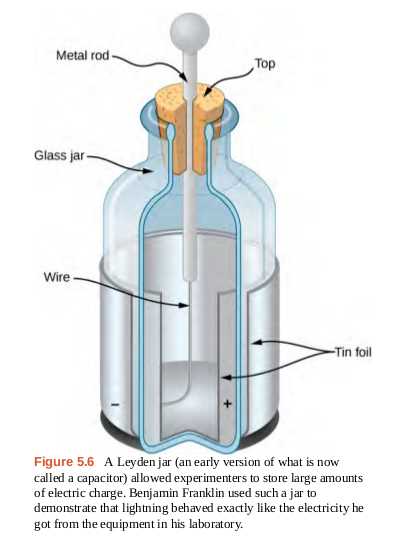
\includegraphics[width=0.3\textwidth]{figures/leyden.png}
\caption{\label{fig:leyden} A Leyden jar was an early version of a capacitor.  Benjamin Franklin guessed that one type of charge moves and another remains stationary, explaining several behaviors of charged objects.}
\end{figure}
\end{frame}

\begin{frame}{Charge, Conductors and Insulators}
The rest of the properties of charge are connected to the development of the structure of the atom, and we will return to this topic at the end of the semeter.
\begin{figure}
\centering
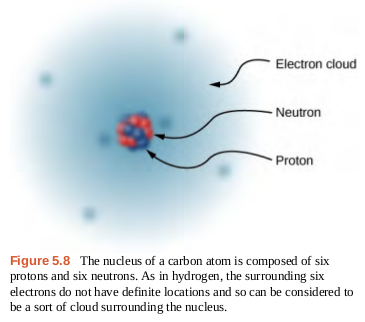
\includegraphics[width=0.5\textwidth]{figures/atom.png}
\caption{\label{fig:atom} A sketch of our current atomic paradigm.}
\end{figure}
\end{frame}

\begin{frame}{Charge, Conductors and Insulators}
Suppose an ion is composed of six protons, eight neutrons, and five electrons.  What is the net charge?
\begin{itemize}
\item A: +1
\item B: 0
\item C: -1
\item D: -2
\end{itemize}
\end{frame}

\begin{frame}{Charge, Conductors and Insulators}
An insulator with a positive charge is held next to a \textit{conductor} (an object in which charge can move around freely).  Which of the following is true?
\begin{itemize}
\item A: The charges in the conductor all remain in place because charge is conserved.
\item B: The negative charges in the conductor move toward the positive charges in the rod.
\item C: The positive charges remain in place but the negative charges move away from the rod.
\item D: The positive charges move toward the rod and the negative charges remain in place.
\end{itemize}
\end{frame}

\begin{frame}{Charge, Conductors and Insulators}
An \textit{insulator} with a net positive charge is held next to an \textit{insulator} with a net negative charge.  Which of the following is true?
\begin{itemize}
\item A: The charges in the conductor all remain in place, and the force is attractive.
\item B: The charges in the conductor all move around until the force is attractive.
\item C: The charges in the conductor all remain in place, and the force is repellent.
\item D: The charges in the conductor all move around until the force is repellent.
\end{itemize}
\end{frame}

\begin{frame}{Coulomb’s Law and Electric Fields}
The boundary conditions of problems can vary depending on the materials involved: \\ \vspace{0.5cm}
\textbf{Insulator}: A material in which there are no free charges available to conduct electricity.  Charges may be fixed in position within an insulator. \\
\textbf{Conductor}: A material in which there are free charges available to conduct electricity.  Charges may not be fixed in position within a conductor. \\
\textbf{Semi-conductor}: A material in which there are free charges available to conduct electricity if certain requirements are met.
\end{frame}

\section{Activity: PhET Simulation of Charges and Fields}

\begin{frame}{Activity: PhET Charges and Fields}
At your tables, go to the following URL: \\ \vspace{0.2cm}
\url{https://phet.colorado.edu/en/simulation/charges-and-fields} \\ \vspace{0.2cm}
Click on the HTML app to get it running.  Notice the following:
\begin{enumerate}
\item This is a 2D coordinate space, and you can activate the grid lines at right, by clicking \textit{grid.}
\item Clicking \textit{values} gives you the measurement scale.
\item Click \textit{electric field}, or make sure it is activated.
\item Verify the length scale with the \textbf{ruler tool}, shaped like a tape measure.  It can be dragged from the box at right.
\end{enumerate}
\end{frame}

\begin{frame}{Activity: PhET Charges and Fields}
\small
\url{https://phet.colorado.edu/en/simulation/charges-and-fields} \\ \vspace{0.2cm}
\textbf{Click and drag a positive charge into the 2D coordinate system.  This is analagous to charging an insulator.}
\begin{enumerate}
\item Drag the yellow tool at the bottom into the space, and use it to measure the field strength.  Notice the units are in V/m and m.
\item Copy to excel the field strength (E) versus distance (r).  Use 25 cm distance increments, and record 15 data points in two columns.
\item In a third column, compute $r^2 E$.
\end{enumerate}
\end{frame}

\begin{frame}{Activity: PhET Charges and Fields}
\small
\url{https://phet.colorado.edu/en/simulation/charges-and-fields} \\ \vspace{0.2cm}
\textbf{Click and drag a positive charge into the 2D coordinate system.  This is analagous to charging an insulator.}
\begin{enumerate}
\item Plot $r^2 E$ vs. $r$.  Do you observe a flat line?  What are some sources of error that contribute to the uncertainty in the slope?
\item Repeat this same exercise, but instead of measuring field strength versus \textit{distance}, measure it in one location, versus \textit{charge.} Take 15 data points in two columns and plot the results in Excel.  What is the slope of the line?  Notice the units of charge are nC.
\end{enumerate}
\textbf{Example data:} See Moodle for sample data drawn from this PhET.
\end{frame}

\begin{frame}{Charge, Conductors and Insulators}
\centering
\textbf{\alert{Charge: the constant of proportionality between the strength of a \textit{field} and the force a field exerts on an \textit{object}.}} \\
\hrulefill
\small
\begin{columns}[T]
\begin{column}{0.5\textwidth}
\alert{Gravity}
\begin{enumerate}
\item Force: $\vec{F} = G \frac{m M}{r^2} \hat{r}$
\item Parameters: $r$ is absolute distance between two objects with masses $m$ and $M$, and the direction is $\hat{r}$
\item \textit{Charge} of one object: $m$
\item \textit{Field felt by that object}: $\vec{G} = G \frac{M}{r^2} \hat{r}$
\item $\vec{F} = m \vec{G}$
\end{enumerate}
\end{column}
\begin{column}{0.5\textwidth}
\alert{Electricity}
\begin{enumerate}
\item Force: $\vec{F} = k \frac{q Q}{r^2} \hat{r}$
\item Parameters: $r$ is absolute distance between two objects with electric charges $q$ and $Q$, and the direction is $\hat{r}$
\item \textit{Charge} of one object: $q$
\item \textit{Field felt by that object}: $\vec{E} = G \frac{Q}{r^2} \hat{r}$
\item $\vec{F} = q \vec{E}$
\end{enumerate}
\end{column}
\end{columns}
\end{frame}

\begin{frame}{Charge, Conductors and Insulators}
\centering
\textbf{\alert{Charge: the constant of proportionality between the strength of a \textit{field} and the force a field exerts on an \textit{object}.}} \\
\hrulefill \\
\small
In the field paradigm, objects with charges \textit{emanate} fields, causing other objects with charge to experience force. \\
\hrulefill \\
\begin{columns}[T]
\begin{column}{0.5\textwidth}
\alert{Gravity} \\
How many \textit{types of charge}, or how many charges, exist under the force of gravity? \\
\textbf{One.} We call it mass.
\end{column}
\begin{column}{0.5\textwidth}
\alert{Electricity} \\
How many \textit{types of charge}, or how many charges, exist under the force of electricity? \\
\textbf{Two.} We call one positive, and one negative.
\end{column}
\end{columns}
\end{frame}

\begin{frame}{Charge, Conductors and Insulators}
\centering
\textbf{\alert{Charge: the constant of proportionality between the strength of a \textit{field} and the force a field exerts on an \textit{object}.}} \\
\hrulefill \\
\small
In the field paradigm, objects with charges \textit{emanate} fields, causing other objects with charge to experience force. \\
\hrulefill \\
In the field paradigm, gravity has one charge (mass), and electricity has two charges (positive and negative). \\
\hrulefill \\
\textbf{There is one fundamental fact that is puzzling.} What about Newton's 2nd law?  Acceleration is not a field, it is a kinematic function.
\begin{equation}
\vec{F}_{\rm net} = m \vec{a}
\end{equation}
Aparently there are \textit{two kinds of mass}: \textbf{inertial} and \textbf{gravitational}.  
\end{frame}

\begin{frame}{Charge, Conductors and Insulators}
\small
\textit{Equivalence principle:} \\ \hrulefill \\
There are \textit{two kinds of mass}: \textbf{inertial} and \textbf{gravitational}, with \textbf{equal value} for a given object. \\ \vspace{0.5cm}
\url{https://en.wikipedia.org/wiki/Equivalence_principle} \\
\hrulefill \\
There is no similar principle for charge.  If the electric force on a charged object is calculated, that force must still be inserted into \textbf{Newton's 2nd Law} to obtain the acceleration, and the inertial mass must be known.
\end{frame}

\section{Conclusion}

\begin{frame}{WAT.}
\centering

\includegraphics[width=0.4\textwidth]{figures/frogs-know-wats.png}
\end{frame}

\begin{frame}{Unit 0 Summary}
\textit{Physics} - $\phi\upsilon\sigma\iota\kappa\acute{\eta}$ - "phusik\'e": \textit{knowledge of nature} \\
from $\phi\acute{\upsilon}\sigma\iota\varsigma$ - "ph\'usis": \textit{nature} \\
\textbf{Reading: Chapters 18 and 19 (for Unit 1)}
\begin{enumerate}
\item Estimation/Approximation
\item Review of concepts from Newtonian mechanics
\begin{itemize}
\item Kinematics and \alert{Newton's Laws}
\item Work-energy theorem, energy conservation
\item Momentum, conservation of momentum
\end{itemize}
\item Charge
\begin{enumerate}
\item Types of charge, charge conservation
\item Couloumb force
\item Electric fields
\end{enumerate}
\end{enumerate}
\end{frame}

\end{document}
